\chapter{Data corpora for research}\label{chap:datasets}
% \begin{epigraphs}
%   \qitem{Data is a precious thing and will last longer than the systems themselves.}{Tim Berners-Lee}% , inventor of the World Wide Web
% \end{epigraphs}
% Use \noindent for the first paragraph after this
%\dtext{The work we do is data-driven and hence datasets play an important role in research. A significant part of the efforts in the CompMusic project and the thesis are to collaborate and develop datasets for use in research. The chapter discusses the datasets developed within the context of CompMusic, by us and other collaborators. The idea is also to discuss how to measure the goodness of a corpus, what data driven research can be done with datasets and what can we learn directly from datasets.}
%
%\dtext{Abstract: Research corpora are representative collections of data and are essential to develop data-driven approaches in Music Information Research (MIR). We address the problem of building research corpora for MIR in Indian art music traditions of Hindustani and Carnatic music, considering several relevant criteria for building such corpora. We also discuss a methodology to assess the corpora based on these criteria and present an evaluation of the corpora in their coverage and completeness. In addition to the corpora, we briefly describe the test datasets that we have built for use in many research tasks. In specific, we describe the tonic dataset, the Carnatic rhythm dataset, the Carnatic \gls{varnam} dataset, and the Mridangam stroke dataset.}

Computational data-driven MIR research requires a well-curated data corpus for training and testing the models. The corpus should meet certain criteria so that the models can be built successfully built and applicable to real-world scenarios. A research corpus is an evolving data collection which is representative of the research domain under study. A good corpus can be built by a single research institute or by crowdsourcing within a community. Regarding MIR research, a research corpus is a representative subset of one or several music genres, since it is nearly impossible to work with all the relevant music pieces. Computational models developed upon this subset can be assumed generalizable to real-world scenarios.

A test dataset is a subset of the research corpus which is designed for a specific research task. In the research task, the test dataset is used to develop and evaluate computational models. For better reproducibility of experiment results, the test dataset is usually fixed or properly versioned.

Building a research corpus is a research problem itself and has been studied in many fields. There are many repositories for the research of speech such as Linguistic Data Consortium\footnote{\url{https://www.ldc.upenn.edu/}}, Librispeech\footnote{\url{http://www.openslr.org/}}, and for the research of musicology such as IMSLP/Petrucci Music Library\footnote{\url{https://imslp.org/}} and MusicBrainz\footnote{\url{https://musicbrainz.org/}}. There have been efforts to compile large collections for MIR or general sound analysis research such as Million Song Dataset \cite{Bertin-Mahieux2011a}, FMA dataset \cite{Defferrard2017}, AcousticBrainz\footnote{\url{https://acousticbrainz.org/}} and Freesound datasets \cite{Fonseca2017}. These music data collections are good resources for developing MIR models on Western Pop music. A systematic way of building a research corpus is essential for the MIR research, and receives attention from the research community. Serra \cite{Serra2014} described a set of criteria to build a MIR research corpus -- Purpose, Coverage, Completeness, Quality and Reusability. We use these criteria to help develop a corpus for automatic assessment of jingju singing pronunciation.

In this chapter, we compile and analyse the research corpus and test datasets for the research of this dissertation. We will discuss the corpus building criteria and evaluation methodologies. Our main focus in this chapter will be jingju music, while other relevant test datasets are also presented. We aim:

\begin{enumerate}[noitemsep]
\item To describe the corpus and the test datasets, emphasizing the research problems and tasks relevant to this thesis.
\item To describe a set of corpus design criteria and methodologies, then use them to evaluate the jingju a cappella singing voice corpus.
\item To present both corpus-level and test dataset-level musically meaning data analysis and visualization.
\end{enumerate}

We mainly emphasize on presenting a scientific approach for corpus building and the evaluation of its coverage and completeness. Apart from the corpus description, the musically meaningful data analysis and visualization is another contribution of this chapter. Finally, the research corpus and test datasets presented in this chapter will be made available for further jingju MIR research.

\section{CompMusic research corpora}\label{sec:ch4:compmusic_corpora}

Although different music genres share some basic concepts such as melody and rhythm, some other important aspects can be described only by considering the musical specificity of that tradition. In the context of CompMusic project, Serra \cite{serra_multicultural_2011} highlighted the needs for culture-specific MIR research corpora to develop approaches which benefit from the essential aspects of the music tradition. 

In CompMusic project, we work with five music traditions of the world which expose different research problems. A significant effort has been put towards the design the research corpora for the relevant problems of the specific musical traditions. In this chapter, we focus mainly on the a cappella singing voice of jingju music, while jingju commercial audio recording \cite{repetto_creating_2014}, lyrics and musical score collections \cite{Repetto2017} have been presented by other researchers of the CompMusic project. The Carnatic and Hindustani research corpora have been described thoroughly by \cite{Srinivasamurthy2014}. The Turkish makam music research corpus has been presented in detail by \cite{Uyar2014a}.

\subsection{Criteria for the creation of research corpora}

Serra \cite{Serra2014} listed five criteria for build culture-specific MIR research corpus:

``Purpose: The first step in the design of a corpus is to define the research problem that wants to be addressed and the research approach that will be used. In CompMusic, we want to develop methodologies with which to extract musically meaningful representations from audio music recordings, mainly related to melody, rhythm, timbre and pronunciation. The approaches are based on signal processing and machine learning techniques; thus the corpus has to be aligned with this purpose.

Coverage: A corpus has to include data representative of all the concepts to be studied and given our quantitative approach, there have to be enough samples of each instance for the data to be statistically significant. For our research we need to have audio recordings, plus appropriate accompanying information, covering the varieties of pronunciation present in the musical culture.

Completeness: In each corpus, every audio recording is complemented by a set of data fields, and the idea of completeness relates to the percentage of fields filled, thus how complete the corpus is. For our corpora, this mainly refers to the completeness of the editorial metadata and the annotations accompanying each audio recording.

Quality: The data has to be of good quality. The audio has to be well recorded and the accompanying information has to be accurate. We have used well-produced recordings whenever possible, and the accompanying information has been obtained from reliable sources and validated by experts.

Reusability: The research results have to be reproducible, and that means that the corpus has to be available for the research community to use. In our case, we have emphasised the use of specific open repositories such as Zenodo.org\footnote{\url{https://zenodo.org/}} that are either already suitable or that can be adapted to our needs."

Central to the jingju a cappella singing corpus is the audio recordings with its annotation. We present this corpus in the next section.

\subsection{Jingju a cappella singing corpus}\label{sec:ch4:jingju_acappella_singing_corpus}

The jingju a cappella singing corpus mainly contains audio recordings, editorial metadata and musical event annotations. All annotated corpus is the content used by signal processing and machine learning approaches.

Given that aria is the natural unit of jingju music, most audio recordings in this corpus are arias. A unique aria might be sung by different singers with different singing levels -- professional or amateur. To facilitate the development of singing voice assessment models, the audio recordings in this corpus are all a cappella version, meaning without instrumental accompaniment. The singer's singing level is most important metadata associated with a recording.

To build the corpus, we consulted jingju professors and musicologists. The main institutional reference is the National Academy of Chinese Theatre Arts (NACTA)\footnote{\url{https://www.nacta.edu.cn/}}, which is the premier institution dedicated to jingju performing training in Beijing, China, and is the only institute of its kind in China that offers both B.A. and M.A. degrees in jingju performing.

We wish to compile recordings sung by both professional and amateur singers from different backgrounds. The professional recording singers are the professors and students of NACTA. The amateur singers are from various sources -- students of jingju associations in non-art universities, amateurs of jingju groups in community activity centers located in Beijing, amateurs of jingju associations located in London and students from several primary schools. We did not keep track the singer information of the amateurs of jingju groups in community activity centers located in Beijing and the students from several primary schools due to that a large number of singers participated in these recording sessions. Otherwise, the singer information of the other recordings is written in the editorial metadata. 

The corpus has been collected in three different stages and thus been split into three parts. The audios in the first part are recorded with the joint effort of two music technology research institutes -- Center for Digital Music, Queen Mary University of London (C4DM) \cite{Black2014} and Music Technology Group, Universitat Pompeu Fabra (MTG-UPF). Additionally, another 15 clean singing recordings separated from the commercial releases have been included in this part. The audios in the second and third parts are recorded by the author of this thesis during his two times research stay in Beijing.

The corpus consists of 2 role-types (dan and laosheng), 121 unique arias with 289 recordings, meaning several arias have been recorded more than once by different singers. The total duration is 13.61 hours. Other information related to the corpus is described in \tabref{table:ch4:general_statistics_jingju_a_cappella_corpus}.

\begin{landscape}
\mbox{}\vfill
\begin{table}[ht]
    \centering
    \begin{tabular}{l|ccccc}
        \toprule
        Role-type & \makecell{\#Unique aria\\(A: amateur,\\P: professional)} & \#Recording & \#Singers & \makecell{\#Total duration\\(hours)} & \makecell{\#Median recording\\duration (minutes)} \\
        \midrule
        dan           & 73 & 171 (A: 79, P: 83) & 14+ & 8.26 & 1.87 \\
        laosheng      & 48 & 118 (A: 67, P: 51) & 13+ & 5.35 & 2.01 \\
        \bottomrule
    \end{tabular}
    \caption{General statistics of the jingju a cappella singing corpus}
    \label{table:ch4:general_statistics_jingju_a_cappella_corpus}
\end{table}
\vfill
\end{landscape}

The editorial metadata associated with each recording has been stored in MusicBrainz, as well as in Zenodo.org. The primary metadata is the name of the aria, the name of the play and the name of the singers. Each entity such as artist, recording, work, in MusicBrainz is assigned a unique MusicBrainz IDentifier (MBID), which helps organize the metadata. The editorial metadata has been entered using simplified Chinese characters and romanization system -- pinyin. 

A large part of the audio recordings has been annotated. The annotations consist of (i) melodic line onset and offset time boundaries and lyrics in simplified Chinese characters, (ii) syllable onset time stamps and pinyin label, (iii) phoneme onset and offset time boundaries and X-SAMPA label (\appref{app:mandarin_sounds}), (iv) labels indicating the melodic lines which contain long syllables and (v) labels indicating special pronunciations. All annotations have been done in Praat speech analysis and annotation tool \cite{boersma_praat_2001}. Two Mandarin native speakers and one jingju musicologist have dedicated to the annotation. The annotation has been verified and corrected twice by the thesis author to ensure its the boundary accuracy and label correctness.

The whole corpus including audio recordings, editorial metadata and audio annotations are easily accessible from Zenodo.org\footnote{\url{https://doi.org/10.5281/zenodo.780559}}\footnote{\url{https://doi.org/10.5281/zenodo.842229}}\footnote{\url{https://doi.org/10.5281/zenodo.1244732}}.

\subsubsection{Recording setup}\label{sec:ch4:recording_setup}

In the first part of the corpus, the information of recording setup for the audios collected by C4DM has not been given in the original release \cite{Black2014}. However, by listening to each of them, we confirmed that the audios from this part included in the corpus are all good quality. Also in this part, the recordings whose names ending with `upf' are recorded in a professional studio with jinghu accompaniment. Singers and jinghu accompanists are placed separately in different recording rooms and used two recording channels to avoid crosstalk. Other recordings whose name ending with `lon' are recorded by using a Sony PCM-50 portable stereo recorder in a classroom with a certain reverberation. Additionally, another collection of 15 clean singings source-separated from commercial recordings contain audible artefacts of the background accompaniment.

For the second part of the corpus, most of the recording sessions have been conducted in professional recording rooms by using professional equipment. We use two recording equipment sets and two recording rooms:

\begin{itemize}[noitemsep]
    \item Set 1: M-Audio Luna condenser microphone + RME Fireface UCX audio interface + Apple GarageBand for Mac DAW;
    \item Set 2: Mojave MA-200 condenser microphone + ART voice channel microphone preamp + RME Fireface 800 audio interface + Adobe Audition 2.0 DAW;
    \item Room 1: The conference room in NACTA's business incubator with reflective walls, carpet-covered floor, conference furniture and medium room reverberation;
    \item Room 2: The sound recording studio in Institute of Automation, Chinese Academy of Science, with acoustic absorption and isolation.
\end{itemize}

Commercial audio recordings are used, or jingju players are invited for accompanying the singing. When commercial audio recordings were used as the accompaniment, singers were recorded while listening to the accompaniment sent through their monitoring headphone. Otherwise, when \textit{jinghu} players were used as the accompaniment, to simultaneously record both singing and \textit{jinghu} without crosstalk, we placed them separately in two different recording rooms and used two recording channels. However, they were still able to have visual communication through a window and monitor each other through headphones.

For the third part of the corpus, the recording sessions are done by using a Sony PCM-50 portable stereo recorder. The professional singings are recorded during the primary school jingju courses. The recording sessions of primary school students are done in three classrooms rather than asking the students to come to the studio. We believe that recording in the classrooms can represent the room acoustic conditions of the actual jingju teaching. The three rooms are (i) a mid-reflected classroom with the hard wall, marble floor, wood tables, chairs and a blackboard; (ii) a high-reflected dancing rehearsal room with mirrors, hard wall and wood floor; (iii) a mid-reflected dancing rehearsal room with carpet floor, mirrors and glass windows. Lastly, the amateurs of jingju groups in community activity centers are recorded in (iv) a high-reflected community entertainment room with marble floor and hard wall.

\subsubsection{Coverage}

A research corpus needs to be representative of the real world in the concepts that are primary to the music culture \cite{Srinivasamurthy2016}. The main concepts of jingju music -- role-type, shengqiang and banshi, are presented previously in \secref{sec:ch2:jingju_music}. The concepts of jingju singing -- syllable and phoneme are the essential units for the pronunciation assessment. In this work, the coverage analysis is presented for role-type, shengqiang, banshi and phoneme. We do not analyse syllable because there are excessive syllable classes in the languages of jingju singing.

The corpus includes the two jingju role-types whose main discipline is singing -- \textit{laosheng} and \textit{dan}. Both professional and amateur singers have been recorded. For \textit{dan} role-type, there are 79 amateur recordings and 83 professional recordings. For \textit{laosheng} role-type, there are 67 amateur recordings and 51 professional recordings (see \tabref{table:ch4:general_statistics_jingju_a_cappella_corpus}).

\begin{table}[ht]
    \centering
    \begin{tabular}{l|cc}
        \toprule
        Role-type & shengqiang & banshi \\
        \midrule
        dan           & \makecell{xipi, erhuang,\\fanxipi, fanerhuang,\\nanbangzi, sipingdiao,\\fansipingdiao, gaobozi,\\handiao} & \makecell{yuanban, manban,\\kuaiban, liushui,\\erliu, kuaisanyan,\\sanyan, pengban,\\shuban, duoban,\\daoban, huilong,\\yaoban, sanban} \\
	    \hline
	    laosheng      & \makecell{xipi, erhuang,\\fanxipi, fanerhuang} & \makecell{yuanban, manban,\\kuaiban, liushui,\\erliu, kuaisanyan,\\zhongsanyan, sanyan,\\daoban, huilong,\\yaoban, sanban} \\
        \bottomrule
    \end{tabular}
    \caption{A list of shengqiang and banshi included in the corpus.}
    \label{table:ch4:shengqiang_banshi_corpus}
\end{table}

The corpus also includes the two main \textit{shengqiang} - \textit{xipi} and \textit{erhuang}, and a few auxiliary ones, such as \textit{fanxipi}, \textit{fanerhuang}, \textit{sipingdiao}, \textit{nanbangzi}.

In terms of \textit{banshi}, the whole range of metered ones is represented in the dataset - \textit{yuanban}, \textit{manban}, \textit{kuaiban}, \textit{erliu}, \textit{liushui}, \textit{sanyan} and its three variations -- \textit{kuaisanyan}, \textit{zhongsanyan} and \textit{mansanyan}. Besides these metered \textit{banshi}, there are a few unmetered ones -- \textit{sanban}, \textit{daoban}, \textit{yaoban} and \textit{huilong}, whose occurrence is very punctual in performance. A list of shengqiang and banshi included in the corpus for \textit{dan} and \textit{laosheng} role-types is shown in \tabref{table:ch4:shengqiang_banshi_corpus}.

\begin{figure}[ht!]
    \centering
    \subfloat[Dan role-type]{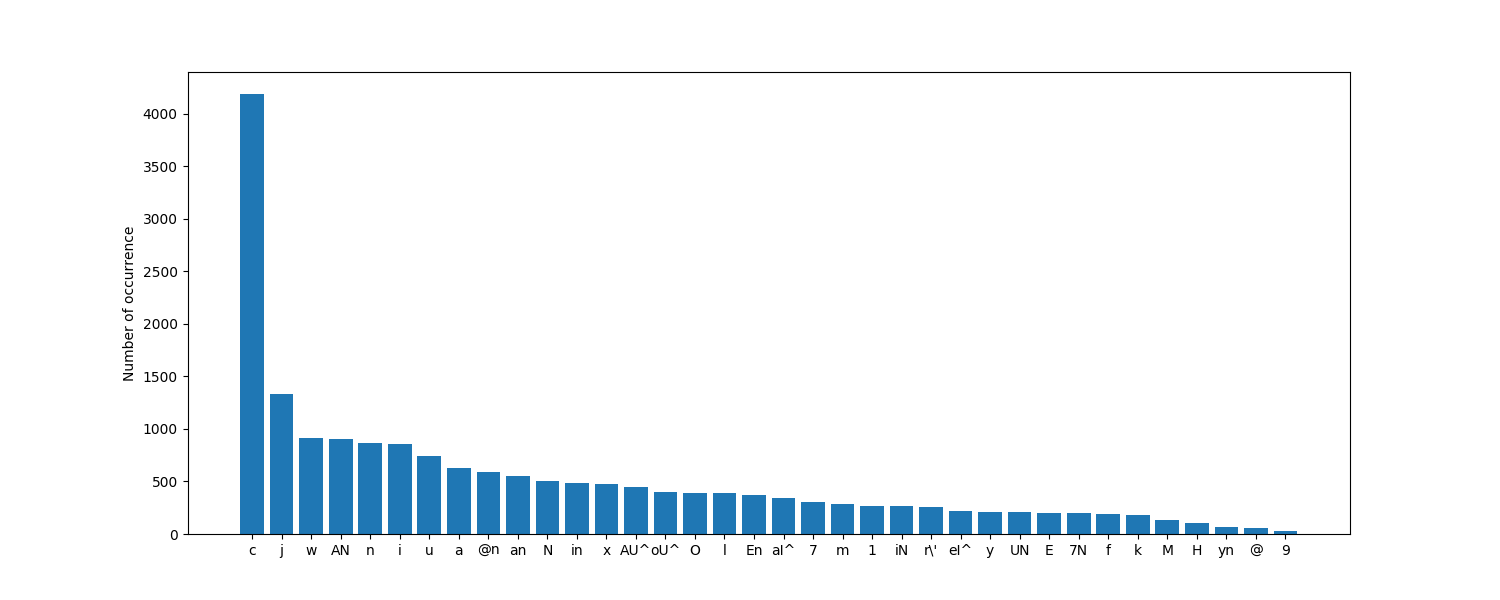
\includegraphics[width=\textwidth]{figs/dstats/dan-number-occurrence.png}
        \label{fig:ch4:number_occurrence_dan}}
    \hfill
    \subfloat[Laosheng role-type]{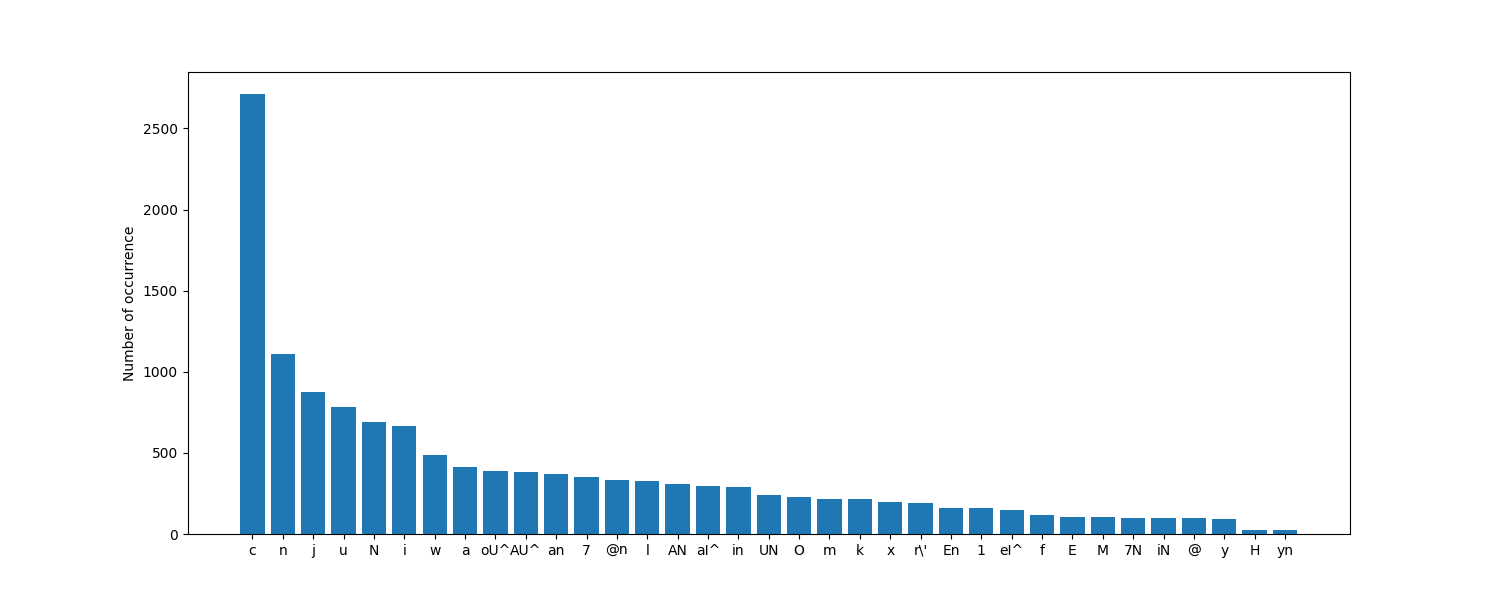
\includegraphics[width=\textwidth]{figs/dstats/laosheng-number-occurrence.png}
        \label{fig:ch4:number_occurrence_laosheng}}
  
    \caption[]{Number of occurrence for each phoneme of dan and laosheng role-types.}
    \label{fig:ch4:number_occurrence}
\end{figure}

\figref{fig:ch4:number_occurrence} represents the number of occurrence for each phoneme for dan and laosheng role-types. We can see that the corpus cover all the phoneme classes for both dan and laosheng role-types, although some phonemes such as ``@", ``yn" have tiny number of occurrence. In all the phoneme classes, ``c", a meta-phoneme class which is merged by all the non-voiced consonants, has the largest number of occurrence. An interesting observation is that the semivowel ``j" has a large number of occurrence because this semivowel is used for both syllable initial and medial vowel. Another large number of occurrence phoneme ``n" is also used for both syllable initial and terminal consonants. Phoneme ``AN" is presented much more in dan singing than in laosheng singing, which indicates that it is preferable to use the syllables constituted with this nasal final in dan singing than in laosheng singing.

\subsubsection{Completeness}

In the context of this dissertation, completeness of the corpus refers to the completeness of the associated metadata and annotation for each recording. As the metadata and annotations are important for training and testing singing assessment machine learning models, they should as complete as possible. 

\begin{table}[ht]
    \centering
    \begin{tabular}{l|cccc}
        \toprule
        Role-type & Metadata & Melodic line & Syllable & Phoneme \\
        \midrule
        dan           & 100\% & \makecell{118/171;\\69\%} 	& \makecell{110/171;\\64.32\%} 	& \makecell{92/171;\\53.8\%} \\
        \hline
        laosheng      & 100\% & \makecell{89/118;\\75.42\%} & \makecell{89/118;\\75.42\%} 	& \makecell{52/118;\\44.06\%} \\
        \bottomrule
    \end{tabular}
    \caption{Metadata and annotations completeness. Table cell format: \#annotated recordings/total recordings; percentage.}
    \label{table:ch4:metadata_completeness}
\end{table}

\begin{table}[ht]
    \centering
    \begin{tabular}{l|cccc}
        \toprule
        Role-type & \#Melodic line & \#Syllable & \#Phoneme \\
        \midrule
        dan           & 1213 	& 9847 	& 18671  	\\
        laosheng      & 893 	& 8239 	& 13378 	\\
        \bottomrule
    \end{tabular}
    \caption{The number of annotated melodic line, syllable and phoneme in the corpus.}
    \label{table:ch4:annotated_number}
\end{table}

The corpus contains the metadata of each recording -- the artist's singing level, the name of the aria, the name of the play and the name of the singing characters. The metadata is 100\% annotated for all recording in the corpus.

The annotations are done in a hierarchical way at melodic line, syllable and phoneme levels. Due to time limits, not all recordings have been annotated. The annotation completeness for each recording in different granularities is shown in \tabref{table:ch4:metadata_completeness}. The number of annotated melodic line, syllable and phoneme are shown in \tabref{table:ch4:annotated_number}.

An important concern in computational research is the reproducibility of the experiments, which requires a corpus openly accessible to the research community. All three parts of the corpus which includes audio, metadata and annotations are stored in Zenodo.org\footnote{\url{https://doi.org/10.5281/zenodo.780559}}\footnote{\url{https://doi.org/10.5281/zenodo.842229}}\footnote{\url{https://doi.org/10.5281/zenodo.1244732}}. The metadata is also organized into releases in MusicBrainz\footnote{\url{https://musicbrainz.org/search?query=jingju\&type=release\&method=indexed}}.

\subsubsection{Dataset analysis}

In this section, we present a corpus-level statistic analysis towards the durations of the melodic line, syllable and phoneme. The goal is to draw musically meaningful insights from the analyses. 

\begin{table}[ht]
    \centering
    \begin{tabular}{l|cc|cc|cc}
        \toprule
        \multirow{2}{*}{Role-type} & \multicolumn{2}{c|}{Melodic line} & \multicolumn{2}{c|}{Syllable} & \multicolumn{2}{c}{Phoneme} \\
        & \makecell{Mean\\Std} & \makecell{Min\\Max} & \makecell{Mean\\Std} & \makecell{Min\\Max} & \makecell{Mean\\Std} & \makecell{Min\\Max} \\
        \midrule
        dan           & \makecell{11.93\\13.85} & \makecell{1.81\\119.69} & \makecell{1.35\\2.66} & \makecell{0.07\\52.66} & \makecell{0.42\\0.75} & \makecell{0.0047\\11.08} \\
        \hline
        laosheng      & \makecell{10.02\\8.86} & \makecell{1.82\\55.92} & \makecell{1.08\\0.84} & \makecell{0.07\\20.63} & \makecell{0.29\\0.62} & \makecell{0.0025\\13.59} \\
        \bottomrule
    \end{tabular}
    \caption{Mean and standard deviation duration, minimum and maximum duration of melodic line, syllable and phoneme (second).}
    \label{table:ch4:mean_std_min_max}
\end{table}

\tabref{table:ch4:mean_std_min_max} shows a basic statistics of duration for melodic line, syllable and phoneme. Some interesting insights can be drawn from the table. Firstly, the mean and standard deviation of melodic line, syllable and phoneme durations of dan role-type are all larger than those of laosheng, which indicates that the length of dan singing regarding melodic line, syllable and phoneme are longer and more varying than that of laosheng. Secondly, the maximum duration of dan melodic line and syllable are more than two times longer than those of laosheng. However, the maximum duration of dan phoneme is shorter than that of laosheng, which indicates that dan role-type tends to prolong the singing syllables and to take more breaths such that a long syllable is split into several phoneme segments by short pauses. Lastly, compared with the mean $<$ 250 ms and standard deviation $<$ 50 ms of the duration of Mandarin speech syllable \cite{wang_syllable_1994}, those of jingju singing voice are at least four times longer and more varying. As we have mentioned in \chapref{chap:probdef}, many singing skills such as ornamentation, breath control, are usually used in interpreting a prolonged syllable. Breath control leads to silences within a syllable; ornamentation leads the variation of the spectral pattern. Long syllable, silences within a syllable and spectral pattern variation bring challenges in developing singing assessment methodologies.

\begin{figure}[ht!]
    \centering
    \subfloat[Dan melodic line]{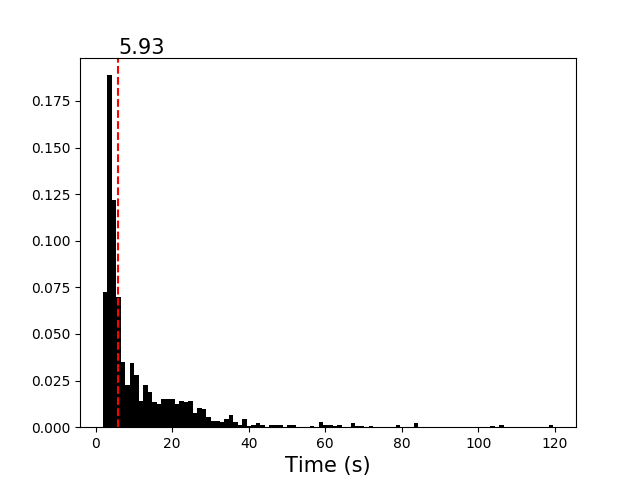
\includegraphics[width=0.32\textwidth]{figs/dstats/dan_melodic_line.png}
        \label{fig:ch4:melodic_line_dan}}
    \subfloat[Dan syllable]{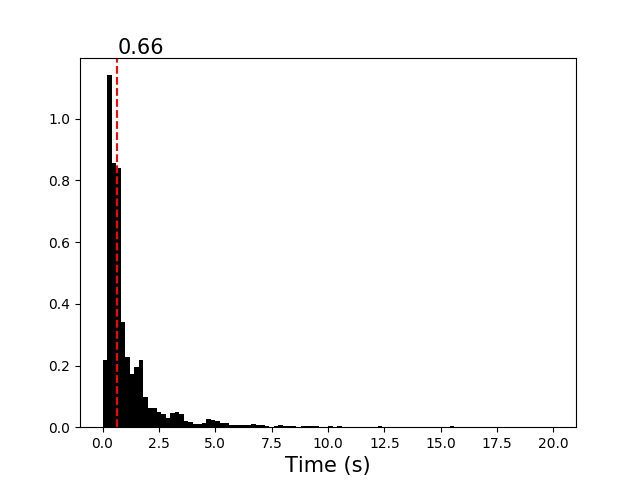
\includegraphics[width=0.32\textwidth]{figs/dstats/dan_syllable.png}
        \label{fig:ch4:syllable_dan}}
    \subfloat[Dan phoneme]{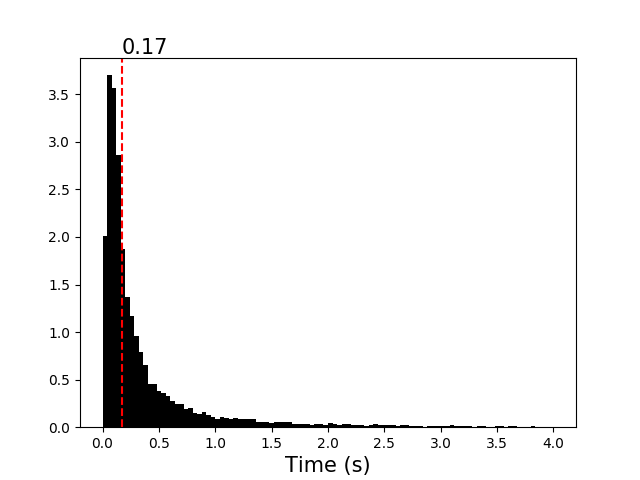
\includegraphics[width=0.32\textwidth]{figs/dstats/dan_phoneme.png}
        \label{fig:ch4:phoneme_dan}}
    \hfill
    \subfloat[Laosheng melodic line]{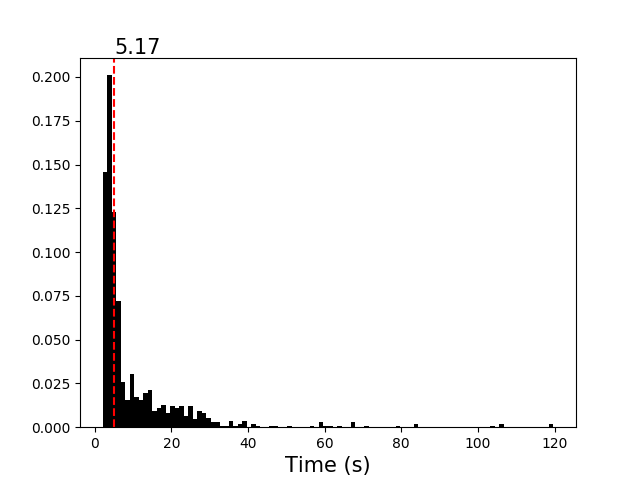
\includegraphics[width=0.32\textwidth]{figs/dstats/laosheng_melodic_line.png}
        \label{fig:ch4:melodic_line_laosheng}}
    \subfloat[Laosheng syllable]{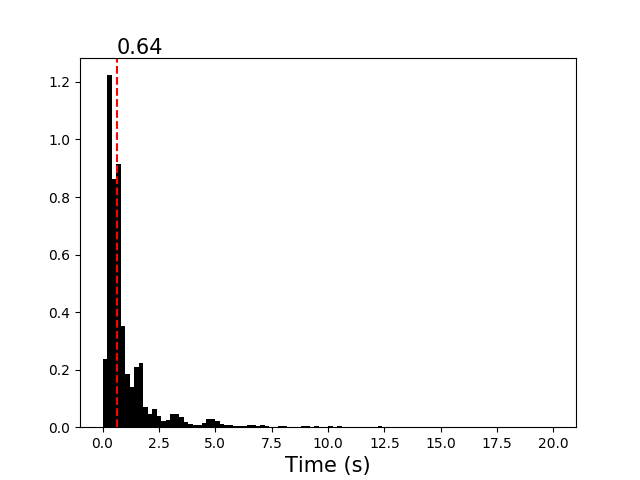
\includegraphics[width=0.32\textwidth]{figs/dstats/laosheng_syllable.png}
        \label{fig:ch4:syllable_laosheng}}
    \subfloat[Laosheng phoneme]{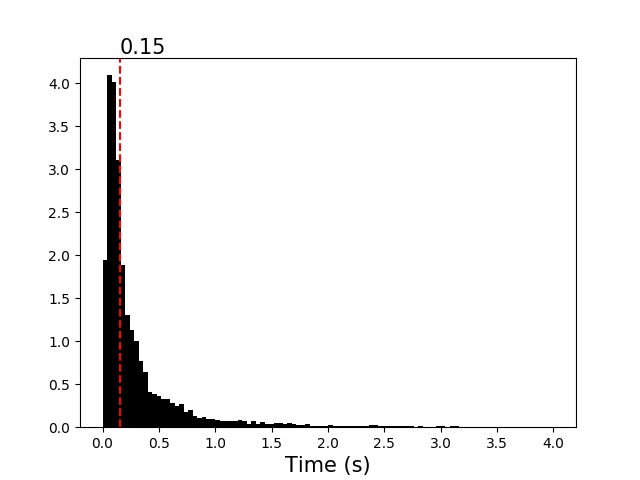
\includegraphics[width=0.32\textwidth]{figs/dstats/laosheng_phoneme.png}
        \label{fig:ch4:phoneme_laosheng}}
  
    \caption[]{Dan and laosheng melodic line, syllable and phoneme duration histograms normalized to unit density. Vertical red dash lines indicate the median duration.}
    \label{fig:ch4:dan_laosheng_histo}
\end{figure}

\figref{fig:ch4:dan_laosheng_histo} shows the duration histograms of melodic line, syllable and phoneme for dan and laosheng role-types. The general shapes of the histogram distribution between dan and laosheng are similar. Although there are prominent peaks on all the histograms, the durations are varied, which can be observed by the extended long-tails on each histogram. For example, the median melodic line duration of dan is 5.93s. However, a significant amount of melodic lines are longer than 10s; the median phoneme duration of laosheng is 0.15s, whereas those phonemes whose durations are more prolonged than 0.4s are not the minority.

\begin{figure}[ht!]
    \centering
    \subfloat[c]{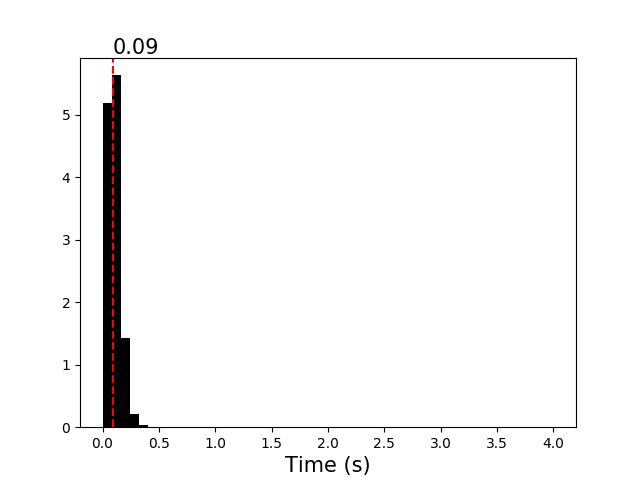
\includegraphics[width=0.43\textwidth]{figs/dstats/dan_c.png}
        \label{fig:ch4:c_dan}}
    \subfloat[l]{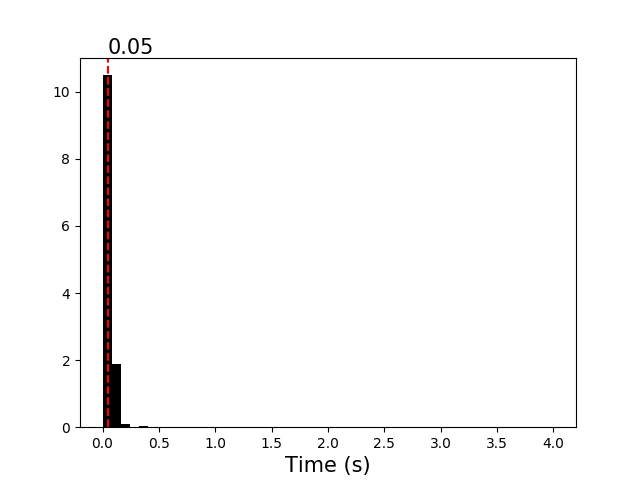
\includegraphics[width=0.43\textwidth]{figs/dstats/dan_l.png}
        \label{fig:ch4:l_dan}}
    \hfill

    \subfloat[N]{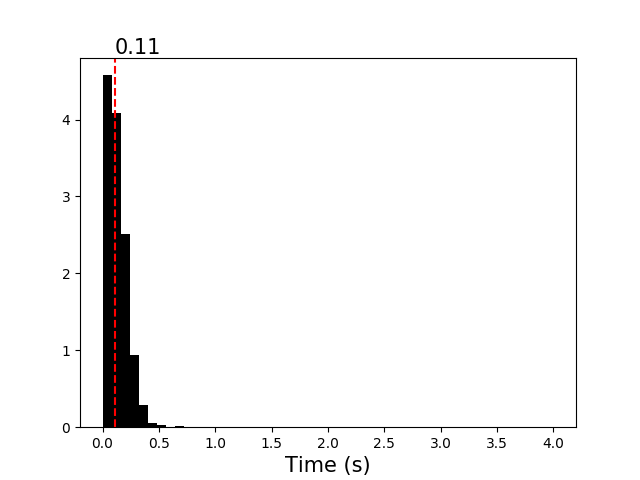
\includegraphics[width=0.43\textwidth]{figs/dstats/dan_N.png}
        \label{fig:ch4:N_dan}}
    \subfloat[@n]{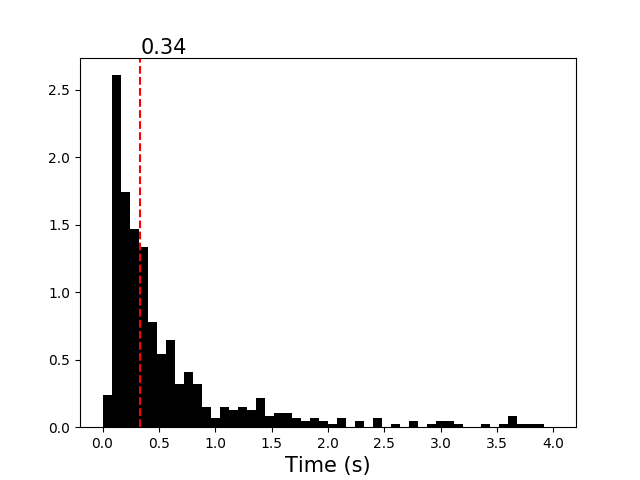
\includegraphics[width=0.43\textwidth]{figs/dstats/dan_@n.png}
        \label{fig:ch4:@n_dan}}
    \hfill
    \subfloat[i]{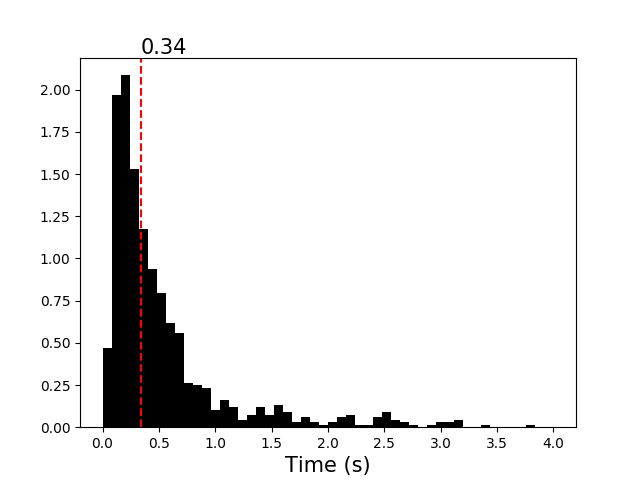
\includegraphics[width=0.43\textwidth]{figs/dstats/dan_i.png}
        \label{fig:ch4:i_dan}}
    \subfloat[a]{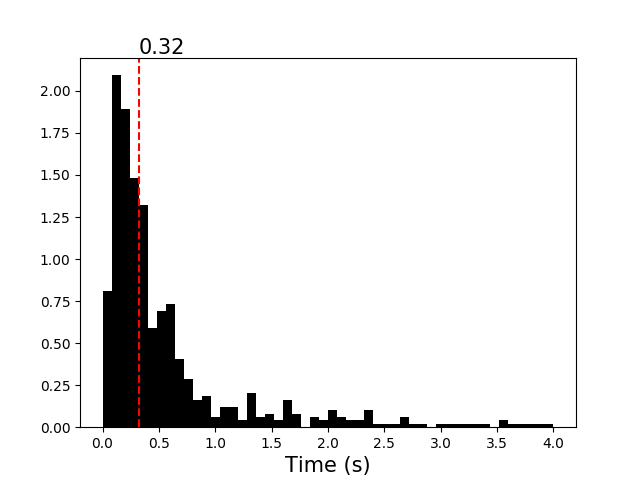
\includegraphics[width=0.43\textwidth]{figs/dstats/dan_a.png}
        \label{fig:ch4:a_dan}}
  
    \caption[]{Dan histograms normalized to the unit density of durations for phonemes c, l, N, @n, i, a. Vertical red dash lines are the median phoneme durations.}
    \label{fig:ch4:dan_histo_phoneme}
\end{figure}

\begin{figure}[ht!]
    \centering
    \subfloat[c]{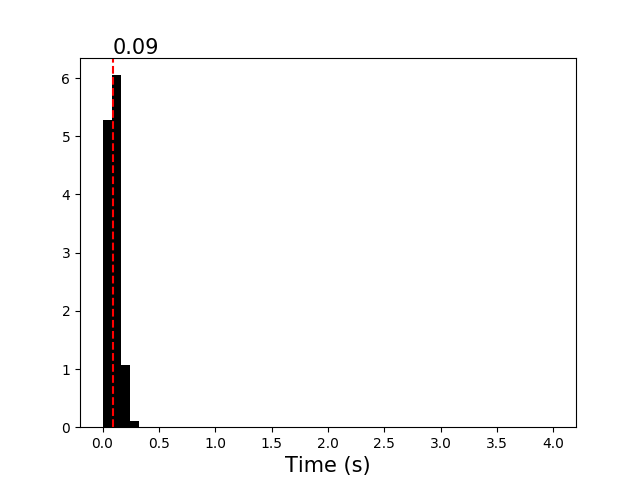
\includegraphics[width=0.43\textwidth]{figs/dstats/laosheng_c.png}
        \label{fig:ch4:c_laosheng}}
    \subfloat[l]{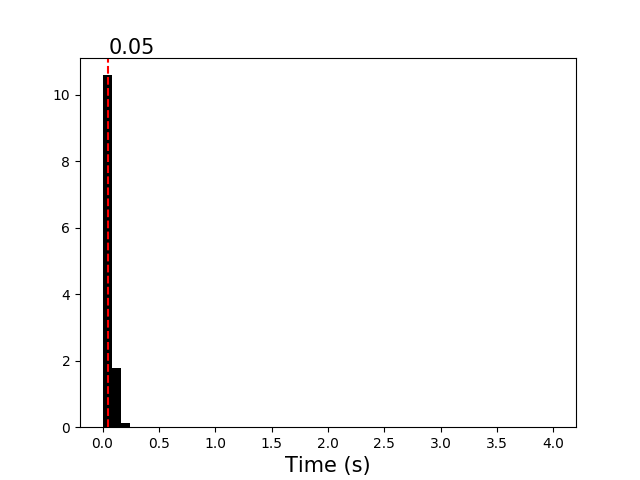
\includegraphics[width=0.43\textwidth]{figs/dstats/laosheng_l.png}
        \label{fig:ch4:l_laosheng}}
    \hfill

    \subfloat[N]{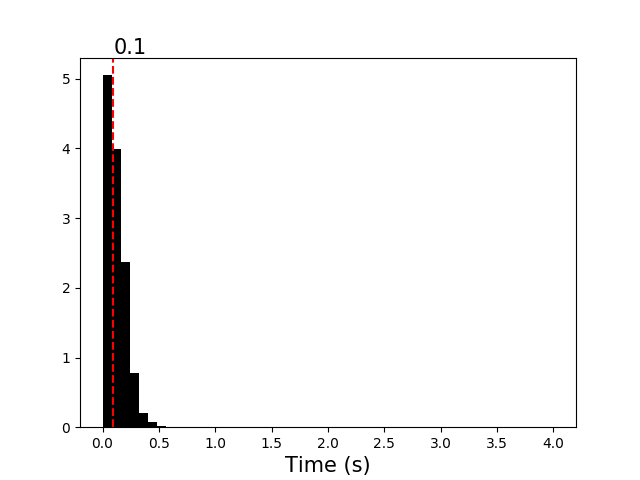
\includegraphics[width=0.43\textwidth]{figs/dstats/laosheng_N.png}
        \label{fig:ch4:N_laosheng}}
    \subfloat[@n]{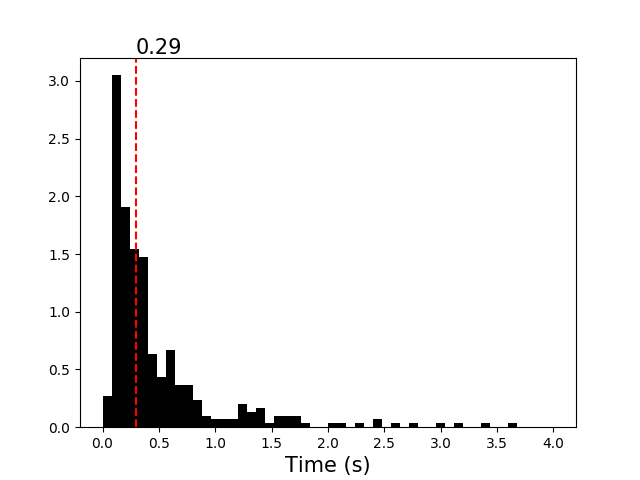
\includegraphics[width=0.43\textwidth]{figs/dstats/laosheng_@n.png}
        \label{fig:ch4:@n_laosheng}}
    \hfill
    \subfloat[i]{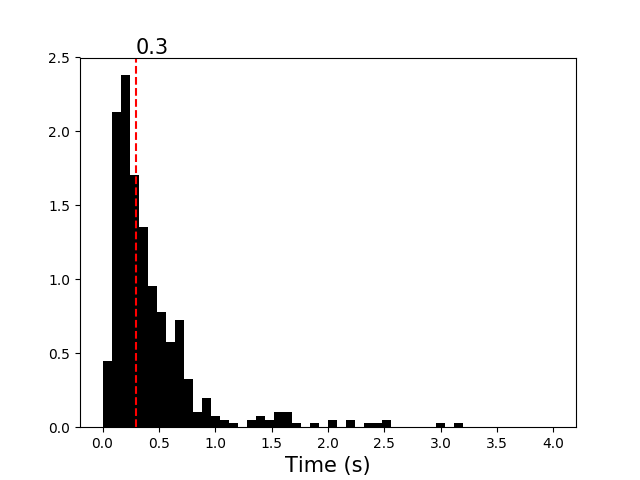
\includegraphics[width=0.43\textwidth]{figs/dstats/laosheng_i.png}
        \label{fig:ch4:i_laosheng}}
    \subfloat[a]{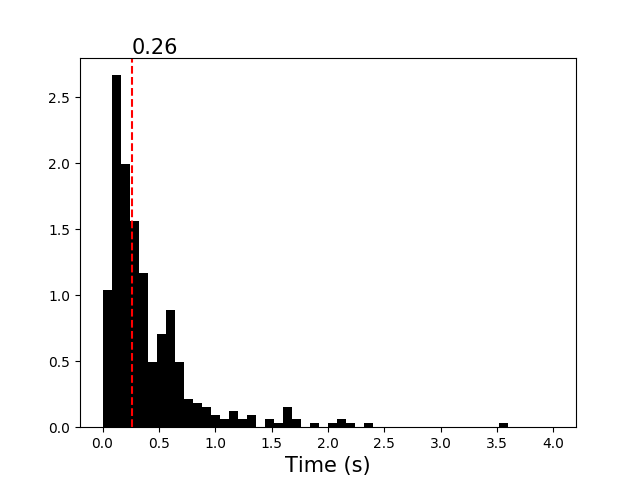
\includegraphics[width=0.43\textwidth]{figs/dstats/laosheng_a.png}
        \label{fig:ch4:a_laosheng}}
  
    \caption[]{Laosheng histograms normalized to the unit density of durations for phonemes c, l, N, @n, i, a. Vertical red dash lines are the median phoneme durations.}
    \label{fig:ch4:laosheng_histo_phoneme}
\end{figure}

\figref{fig:ch4:dan_histo_phoneme} and \figref{fig:ch4:laosheng_histo_phoneme} show the histograms of durations for the individual phoneme. The phonemes which we are selected to show are c, l, N, @n, i, a, in X-SAMPA format. c is an ensemble phoneme class of non-voiced consonants; l is a voiced phoneme; N is a terminal consonant; @n is a diphthong used as the central vowel in a syllable; i and a are single vowels also used as the central vowel in a syllable. Again, the general shapes of the histogram distribution between dan and laosheng are similar. The median duration of the individual phoneme of dan is longer than that of laosheng except for syllable initial consonants -- c and l. The duration of initial consonants does not vary much. However, the central vowels show a large duration variation since which are the primary part of a syllable sung by a singer in a prolonged way.

\section{Test datasets}\label{sec:ch4:test_datasets}
The test datasets are designed for special research tasks. There are several test datasets built in CompMusic for different musical traditions\footnote{\url{http://compmusic.upf.edu/datasets}}. We describe in this section only the test datasets for the tasks of automatic assessment of jingju singing pronunciation.

\subsection{Dataset for automatic syllable and phoneme segmentation}\label{sec:ch4:dataset_segmentation}

Automatic syllable and phoneme segmentation task require the data having syllable and phoneme time boundary and label annotations. Thus, we select the recordings with associated annotations in the corpus to form the test datasets. Two datasets are prepared -- ASPS\textsubscript{1} and ASPS\textsubscript{2}. ASPS\textsubscript{1} will be used for setting the baseline syllable and phoneme segmentation model, while ASPS\textsubscript{2} will be applied for searching an efficient state of the art syllable segmentation model.

ASPS\textsubscript{1} is a subset of the jingju a cappella singing corpus. The recordings in this dataset are selected from all three parts of the corpus. ASPS\textsubscript{1} contains two jingju role-types: \textit{dan} and \textit{laosheng}. 

\begin{table}[ht]
    \centering
    \begin{tabular}{l|cccc}
        \toprule
        & \#Recordings & \#Melodic line & \#Syllables & \#Phonemes \\
        \midrule
        Train           & 56 & 214 & 1965 & 5017 \\
        Test               & 39 & 216 & 1758 & 4651  \\
        \bottomrule
    \end{tabular}
    \caption{Statistics of the ASPS\textsubscript{1} test dataset.}
    \label{table:ch4:detailInfoDataset_asps_1}
\end{table}

The dataset contains 95 recordings split into train and test sets (table \ref{table:ch4:detailInfoDataset_asps_1}). The recordings in the test set only include student imitative singing. The corresponding teacher's demonstrative recordings can be found in the train set, which guarantees that the coarse syllable/phoneme duration and labels are available as a priori information being used in model testing. Recordings are pre-segmented into melodic line units. The syllable/phoneme ground truth boundaries (onsets/offsets) and phoneme labels are manually annotated. 29 phoneme categories are annotated, which include a silence category and a non-identifiable phoneme category, e.g. throat-clearing sound. The category table can be found in the Github page\footnote{\label{ft:github}\url{https://github.com/ronggong/interspeech2018_submission01}}. The dataset is publicly available\footnote{\url{https://doi.org/10.5281/zenodo.1185123}}.

\begin{table}[ht]
    \centering
    \begin{tabular}{l|ccc}
        \toprule
        & \#Recordings & \#Melodic line & \#Syllables \\
        \midrule
        Train           & 85 & 883 & 8368  \\
        Test               & 15 & 133 & 1203  \\
        \bottomrule
    \end{tabular}
    \caption{Statistics of the ASPS\textsubscript{2} test dataset.}
    \label{table:ch4:detail_info_jingju_dataset_asps_2}
\end{table}

ASPS\textsubscript{2} test dataset is also a subset of the jingju a cappella singing corpus. It also includes recordings of dan and laosheng role-types. ASPS\textsubscript{2} contains 100 recordings manually annotated for each syllable onset. The syllable segmentation evaluation will be conducted on each melodic line which has been pre-segmented manually. The statistics and train-test sets split are shown in table \ref{table:ch4:detail_info_jingju_dataset_asps_2}. It is worth to mention that the artists, recording rooms and recording equipment used for the test set is completely different from the training set. This train-test split setup avoids the artist/room/equipment filtering effects which might be happening in the evaluation process\cite{Flexer2010}. The musical score is also included in this dataset, which provides the syllable duration prior information for the evaluation. This dataset is openly available\footnote{\url{https://doi.org/10.5281/zenodo.1341070}\label{fn:jingju_dataset}}.

As it has been mentioned in \secref{sec:ch3:challenges}, pronunciation is a subconcept of the timbre, and in a signal point of view, timbre is related to the spectral envelope shape and the time variation of spectral content. In the following of this section, we show several spectrogram examples of various phoneme categories -- syllable initial non-voiced consonant, voiced consonant, medial vowel, central vowel and syllable terminal consonant, and the transition between two phonemes such as from syllable initial non-voice consonant to media vowel and from central vowel to syllable terminal consonant.

\begin{figure}[ht!]
    \centering
    \subfloat[Mel spectrogram of syllables ``hua, jie, shen".]{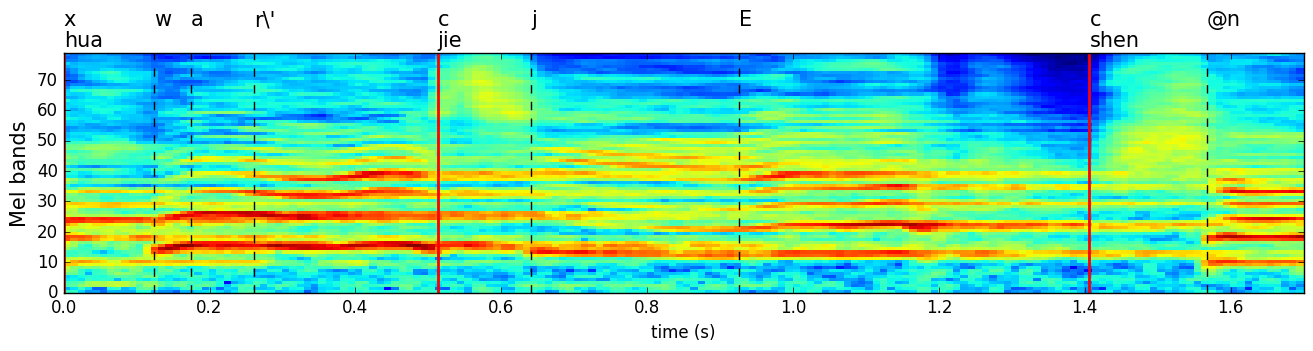
\includegraphics[width=\textwidth]{figs/dstats/spectro_hua_jie_shen.png}
        \label{fig:ch4:hua_jie_shen}}
    \hfill
    \subfloat[Mel spectrogram of syllables ``lai, li, hua".]{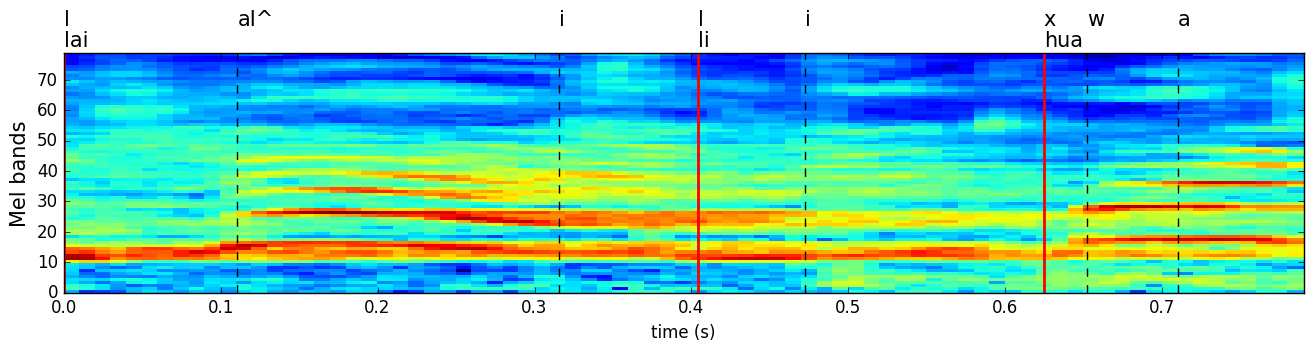
\includegraphics[width=\textwidth]{figs/dstats/spectro_lai_li_hua.png}
        \label{fig:ch4:lai_li_hua}}
    \hfill

    \subfloat[Mel spectrogram of syllables ``da, dan, ren".]{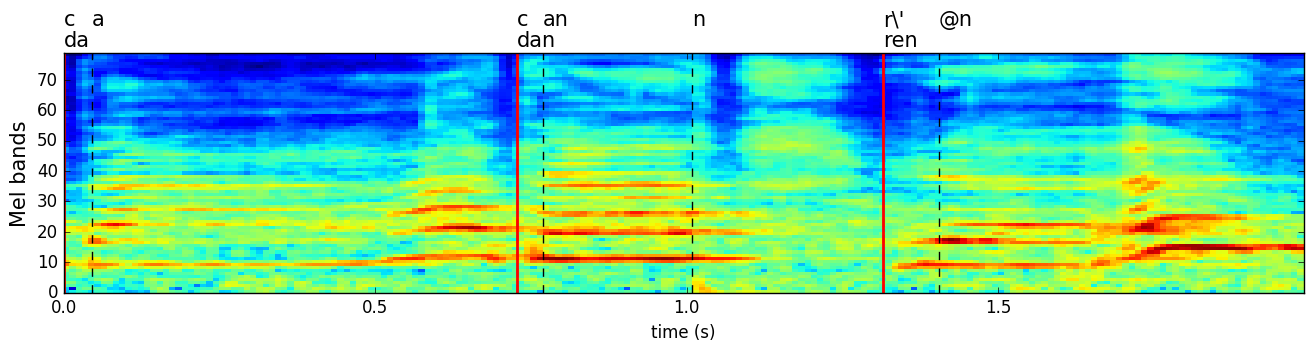
\includegraphics[width=\textwidth]{figs/dstats/spectro_da_dan_ren.png}
        \label{fig:ch4:da_dan_ren}}
  
    \caption[]{Three examples of syllablic Mel spectrogram. Vertical red solid lines are syllable onsets; vertical black dash lines are phoneme onsets.}
    \label{fig:ch4:task1_visualization}
\end{figure}

\figref{fig:ch4:task1_visualization} show three Mel spectrograms of singing syllable sequence, each of which consists of three syllables. We focus the analysis of the middle syllable of each sequence such that the transition between the first and second syllables and the transition between the second and third syllables can be visualized easily. 

The pinyin of middle syllable in \figref{fig:ch4:hua_jie_shen} is ``jie", which consists of three phonemes -- non-voiced consonant ``c", medial vowel ``j" and central vowel ``E". The spectrogram pattern of the non-voiced consonant ``c" can be distinguished easily from ``j" and ``E" by the high-frequency noise-like content since the consonant ``c" is an affricate. The spectrogram pattern of the central vowel ``E" contains more regular harmonic pattern than the medial vowel ``j". However, the difference between the patterns of ``j" and ``E" is not that obvious to discriminate.
 
The pinyin of the middle syllable in \figref{fig:ch4:lai_li_hua} is ``li", which consists of two phonemes -- syllable initial voiced consonant ``l" and the central vowel ``i". The difference of spectrogram pattern between these two phonemes can be hardly distinguished.

The pinyin of the middle syllable in \figref{fig:ch4:da_dan_ren} is ``dan", which consists of three phonemes -- syllable initial non-voiced consonant ``c", central vowel ``an" and syllable terminal consonant ``n". The consonant ``c" is a short non-voiced stop which doesn't contain harmonics. Thus, it can be distinguished easily from the central vowel ``an". The syllable terminal consonant ``n" doesn't contain any higher harmonics. Therefore, it can be distinguished easily as well from the central vowel ``an".

Given the analysis of the above three spectrogram examples, we can design the methodologies for the syllable and phoneme segmentation task in an intuitive way. Firstly, as most of the phoneme categories can be distinguished between each other except for medial vowel-central vowel and voiced consonant-central vowel, we can develop the segmentation algorithm based on the discrimination between phonemes. Secondly, as there are usually obvious spectrogram pattern transitions between phoneme segments, we can also devise the algorithm based on the detection of these transitions. The segmentation algorithms development and evaluation will be presented in detail in the next Chapter.

\subsection{Dataset for mispronunciation detection}\label{sec:ch4:dataset_mispronunciation}

As we have mentioned in \secref{sec:ch3:mispronunciation}, we consider only two types of mispronunciation in jingju singing -- the mispronunciation of special pronunciation and that of jianzi. The first type of mispronunciation -- special pronunciation, is that some written characters in jingju singing pieces should be pronounced differently than in Mandarin Chinese, however, the student doesn't pronounce them correctly as in teacher's demonstrative singing. The second type of mispronunciation -- jianzi, is that certain rounded syllables (团子, pinyin: tuanzi) in jingju singing pieces can be altered to pronounce as the pointed sounds (尖子, pinyin: jianzi), however, the student doesn't pay attention and still pronounce them as rounded syllables. 

In the actual jingju teaching scenario, the teacher's demonstrative singing pieces are given, thus we can identify in advance those special pronounced and jianzi written characters in the pieces. After we obtain the student's imitative singing pieces, the detection process can be carried out only on those special pronounced and jianzi written characters. To this end, we need a model which either can transcribe orthographically each singing syllables considering the special pronunciations and jianzi, or can distinguish between the standard Mandarin pronunciations and the special pronunciations/jianzi. Either way, we need a test dataset where the special pronounced syllables and jianzi are annotated orthographically in pinyin and in phoneme using X-SAMPA format.

\begin{table}[ht]
    \centering
    \begin{tabular}{l|ccccc}
        \toprule
        & \makecell{\#Melodic\\line} & \#Syl. & \makecell{\#Special\\pronunciation} & \#jianzi & \#Phn. \\
        \midrule
        Train           & 662 & 5797 & 463 & 41 & 15287 \\
        Test               & 345 & 3106 & 356 & 13 & 7561 \\
        \bottomrule
    \end{tabular}
    \caption{Statistics of the MD test dataset. Syl.: syllable; Phn.: phoneme.}
    \label{table:ch4:detailInfoDataset_md}
\end{table}

The Mispronunciation Detection -- MD test dataset is annotated for the above purpose. MD is a subset of the jingju a cappella singing corpus. The recordings in this dataset are selected mainly from the part 1 and 2 of the corpus. \tabref{table:ch4:detailInfoDataset_md} shows the statistics of the MD test dataset which are split into train and test parts, and the test part contains only the recordings of amateur singings. As we can see from the table, the occurrence of the special pronounced syllables is much larger than jianzi. Most importantly, in the test part of the MD dataset, according to the teacher's demonstrative recordings, there are in total 451 syllables of special pronunciation and 50 syllables of jianzi should be pronounced correctly by the students. However, in the actual recordings of the test part of the MD dataset, there are 102 syllables of special pronunciation and 37 syllables of jianzi which have been mispronounced, and 349 syllables of special pronunciation and 13 syllables of jianzi which have been pronounced correctly. These mispronounced syllables are labeled manually by comparing the annotation of the test recording and that of the corresponding teacher's demonstrative recording. For example, if in the teacher's recording, there is a special pronunciation /ngo/ for the syllable ``wo”, however, in the amateur's recording, the corresponding syllable is still pronounced as /wo/, this syllable is labeled as a mispronunciation.


\begin{figure}[ht!]
\makebox[\textwidth][c]{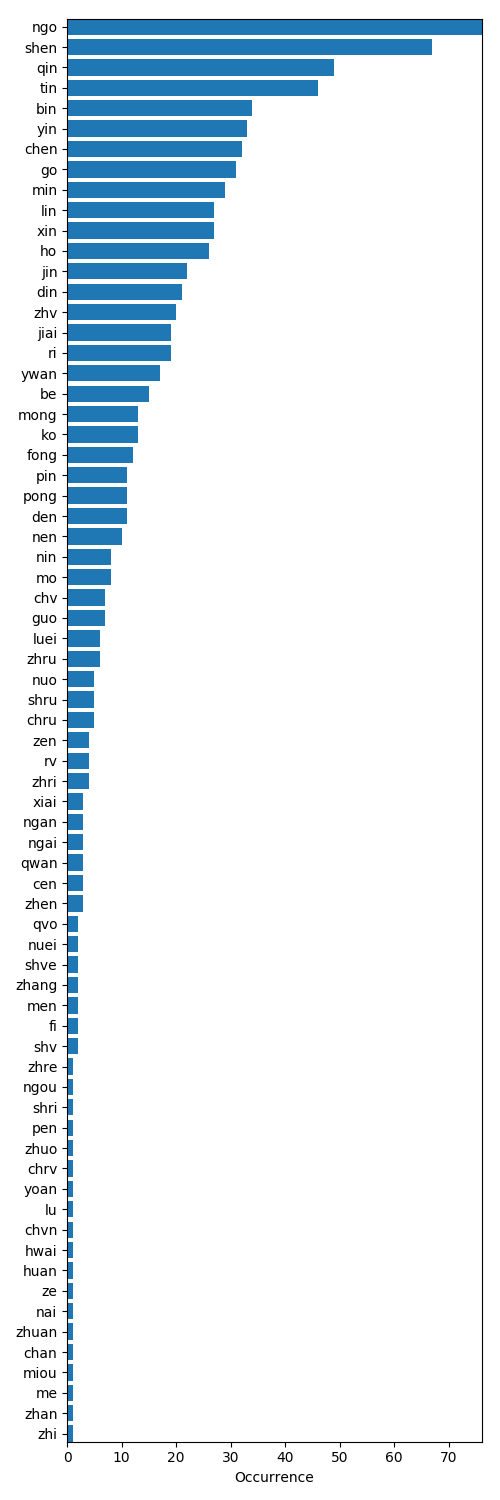
\includegraphics[width=0.6\textwidth]{figs/dstats/occurrence_special.png}}
\caption{The occurrence of each special pronounced syllable.}
\label{fig:ch4:occurrence_special}
\end{figure}

\figref{fig:ch4:occurrence_special} shows the occurrence of each special pronounced syllables in MD dataset. The most frequently occurred syllables are /ngo (我), shen, qin, tin, bin, yin, chen, go, min, lin, xin, ho/. The pronunciation /ngo/ is altered from /wo/ in standard Mandarin by changing the semivowel /w/ to the nasal consonant /ng/. The syllables /go/ and /ho/ are altered from /ge/ and /he/ in standard Mandarin by changing the vowel /e/ to /o/. The other syllables mentioned above are the alteration from velar nasal to alveolar nasal, for example, changing from /eng/ and /ing/ to /en/ and /in/. The full table of the alteration from Mandarin pronunciation to the special pronunciation appeared in the MD test dataset is presented in \tabref{tab:app:special_pronun}.

\begin{figure}[ht!]
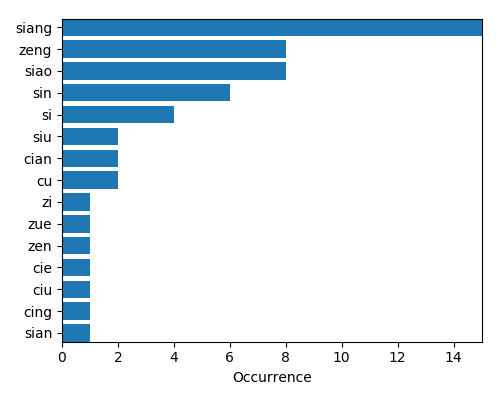
\includegraphics[width=\textwidth]{figs/dstats/occurrence_jianzi.png}
\caption{The occurrence of each jianzi syllable.}
\label{fig:ch4:occurrence_jianzi}
\end{figure}

\figref{fig:ch4:occurrence_jianzi} shows the occurrence of each jianzi in MD dataset. As we have mentioned in \secref{sec:ch2:jiantuanzi}, the rule of this pronunciation alteration is /j, zh/ -> /z/, /q, ch/ -> /c/, /x, sh/ -> /s/. For example, the pronunciation /siang/ is altered from /xiang/, and /zeng/ is altered from /zheng/. The full table of rounded syllables to the special pronunciation appeared in the MD test dataset is presented in \tabref{tab:app:jianzi}.

\subsection{Dataset for pronunciation and overall quality similarity measures}

The test dataset for the task of pronunciation and overall quality similarity measures (POQSM) needs to have phoneme-level onset and offset time boundary and label annotation. These recordings are also a subset of the jingju a cappella singing corpus. The phoneme segments of the dataset are randomly split into the train, validation and test sets, except that we deliberately use the recordings of the amateurs of jingju groups in community activity centers (see \secref{sec:ch4:jingju_acappella_singing_corpus} for the information of the recording artists of the corpus) as the amateur part of the test set. The purpose of using this special amateur part of the test set is to avoid artist and room filtering effects by checking if the trained assessment model overfits on certain singers or the acoustic room conditions of the train and validation sets.

\begin{landscape}
\mbox{}\vfill
\begin{table}[ht!]
\centering
\begin{tabular}{l|c|c|c|c}
\toprule
           & \makecell{\#Professional\\phonemes} & \makecell{\#Amateur\\phonemes} & Professional singers                                        & Amateur singers                                 \\
\midrule
Train      & 6888                     & 5673                & \multirow{3}{*}{\makecell{Adult\\conservatory students\\or graduates}} & \multirow{2}{*}{Mainly primary school students} \\
\cline{1-3}
Validation & 1733                     & 1429                &                                                             &                                                 \\
\cline{1-3}\cline{5-5}
Test       & 2167                     & 2021                &                                                             & Adult amateur singers \\
\bottomrule
\end{tabular}
\caption{POQSM test dataset split, numbers of the professional and amateur singing phonemes and the source of the professional and amateur singers.}
\label{tab:ch4:exp_dataset_poqsm}
\end{table}
\vfill
\end{landscape}

We consider the fact that, after dataset splitting, the train, validation and test sets would contain both professional and amateur phoneme segments. Additionally, the amateur part of the train and validation sets mainly include the phoneme segments of the primary school students, while that of the test set contains exclusively the segments of the adult singers recorded in a different room (see the room iv in section \ref{sec:ch4:recording_setup}). This special split of the test set would verify the artist or room filtering effect of the assessment model \cite{Flexer2010}. Please check table \ref{tab:ch4:exp_dataset_poqsm} for the phoneme numbers and the singers in each split. For the detailed information on the phoneme numbers per phoneme class and recording file names used for each split, please consult this link\footref{foot:zenodo_dlfm2018}. The test dataset can be download in this link\footnote{\url{https://doi.org/10.5281/zenodo.1287251}\label{foot:zenodo_dlfm2018}}.

An example of spectrogram visualization between teacher and student singing melodic line has been presented already in \secref{sec:ch3:char_singing}. In such an example, although the student does not commit any mispronunciation, there still exists a significant pronunciation quality and an overall quality gap between her singing and the teacher singing. Building a pronunciation and overall quality similarity model can help detect the relevant singing problems automatically apart from mispronunciation.
